
%\documentclass[11pts,a4paper,amsmath,amssymb,floatfix]{article}%{report}%{book}
\documentclass[12pts,a4paper,amsmath,amssymb,floatfix]{article}%{report}%{book}
\usepackage[pdftex,colorlinks=true,urlcolor=blue,citecolor=blue]{hyperref}
\usepackage{graphicx} 
\usepackage{wrapfig,pdfpages}% Include figure files
%\usepackage{dcolumn,enumerate}% Align table columns on decimal point
\usepackage{enumerate}%,enumitem}% Align table columns on decimal point
\usepackage{bm,dpfloat}% bold math
%\usepackage[pdftex,bookmarks,colorlinks=true,urlcolor=rltblue,citecolor=blue]{hyperref}
\usepackage{amsfonts,amsmath,amssymb,stmaryrd,indentfirst}
\usepackage{times,psfrag}
\usepackage{natbib}
\usepackage{color}
\usepackage{units}
\usepackage{rotating}
\usepackage{multirow}

%%% For restarting section numbering
\makeatletter
\@addtoreset{section}{part}
\def\@part[#1]#2{%
    \ifnum \c@secnumdepth >\m@ne
      \refstepcounter{part}%
      \addcontentsline{toc}{part}{\thepart\hspace{1em}#1}%
    \else
      \addcontentsline{toc}{part}{#1}%
    \fi
    {\parindent \z@ \raggedright
     \interlinepenalty \@M
     \normalfont\centering
     \ifnum \c@secnumdepth >\m@ne
       \LARGE\bfseries \partname\nobreakspace\thepart
       \par\nobreak
     \fi
     \huge \bfseries #2%
     \markboth{}{}\par}%
    \nobreak
    \vskip 3ex
    \@afterheading}
\renewcommand\partname{Part}
\makeatother



\usepackage{pifont}
\usepackage{subfigure}
\usepackage{subeqnarray}
\usepackage{ifthen}

\usepackage{supertabular}
\usepackage{moreverb}
\usepackage{listings}
\usepackage{palatino}
%\usepackage{doi}
\usepackage{longtable}
\usepackage{float}
\usepackage{perpage}
\MakeSorted{figure}
%\usepackage{pdflscape}
\usepackage{soul} %% use \hl to higlight text

\usepackage{framed}
\definecolor{shadecolor}{gray}{0.9}
%\usepackage{booktabs}
%\newcommand{\ra}[1]{\renewcommand{\arraystretch}{#1}}


\definecolor{rltblue}{rgb}{0,0,0.75}


%\usepackage{natbib}
\usepackage{fancyhdr} %%%%
\pagestyle{fancy}%%%%
% with this we ensure that the chapter and section
% headings are in lowercase
%%%%\renewcommand{\chaptermark}[1]{\markboth{#1}{}}
\renewcommand{\sectionmark}[1]{\markright{\thesection\ #1}}
\fancyhf{} %delete the current section for header and footer
\fancyhead[LE,RO]{\bfseries\thepage}
\fancyhead[LO]{\bfseries\rightmark}
\fancyhead[RE]{\bfseries\leftmark}
\renewcommand{\headrulewidth}{0.5pt}
% make space for the rule
\fancypagestyle{plain}{%
\fancyhead{} %get rid of the headers on plain pages
\renewcommand{\headrulewidth}{0pt} % and the line
}

\def\newblock{\hskip .11em plus .33em minus .07em}
\usepackage{color}

%\usepackage{makeidx}
%\makeindex

\setlength\textwidth      {16.cm}
\setlength\textheight     {22.6cm}
\setlength\oddsidemargin  {-0.3cm}
\setlength\evensidemargin {0.3cm}

\setlength\headheight{14.49998pt}
\setlength\topmargin{0.0cm}
\setlength\headsep{1.cm}
\setlength\footskip{1.cm}
\setlength\parskip{0pt}
\setlength\parindent{0pt}


%%%
%%% Headers and Footers
\lhead[] {\text{\small{EG501V -- Computational Fluid Dynamics}}}
\rhead[\text{\small{Assignment 2017/18}}]{Assignment 2017/18}
\lfoot[]{CFD}
\rfoot[\thepage]{\thepage}
\renewcommand{\headrulewidth}{0.8pt}


%%%
%%% space between lines
%%%
\renewcommand{\baselinestretch}{1.5}

\newcommand{\frc}{\displaystyle\frac}
\newcommand{\red}{\textcolor{red}}
\newcommand{\blue}{\textcolor{blue}}
\newcommand{\green}{\textcolor{green}}
\newcommand{\purple}{\textcolor{purple}}
\newcommand{\eg}{{\it e.g., }}
\newcommand{\ie}{{\it i.e., }}
\newcommand\Rey{\mbox{\textit{Re}}\,\,}
\newcommand\bfr[1]{\textcolor[rgb]{1,0.00,0.00}{\textbf{\textsf{#1}}}}
\newcommand\ra{$\rightarrow$}
\newcommand\cm{\textcolor[rgb]{0.00,0.50,0.00}{\checkmark}\,\,}
\newcommand{\vv}{V$\&$V}



%%%%%%%%%%%%%%%%%%%%%%%%%%%%%%%%%%%%%%%%%%%
%%%%%%                              %%%%%%%
%%%%%% END OF THE NOTATION SECTION  %%%%%%%
%%%%%%                              %%%%%%%
%%%%%%%%%%%%%%%%%%%%%%%%%%%%%%%%%%%%%%%%%%%


% Cause numbering of subsubsections.
%\setcounter{secnumdepth}{8}
%\setcounter{tocdepth}{8}

\setcounter{secnumdepth}{4}%
\setcounter{tocdepth}{4}%


\begin{document}

\begin{center}
  \Large{\bf Final CFD Assignment}
\end{center}


\section{Introduction} 
High-density polyethylene (HDPE) is the third largest commodity plastic material produced in the world (after PVC and PP) with annual production of 51.33 MMT (2016) and worth of approximately USD 64 billions. HDPE resin is used in a wide range of applications from food and beverage packaging to corrosion- and thermal-resistant pipes. There are several industrial patented technology processes to produce HDPE worldwide, \eg 'Chevron-Philips Slurry Loop', 'Lyondell-Basell Ziegler Slurry Process', 'DOW Chemical Solution Process', Univation's 'UNIPOL Swing Process' (Fig.~\ref{HDPE_Plant}) etc.

\medskip
The aim of this practical is to prepare preliminary fluid flow designs of the ethylene flow stream prior to the polymerisation reactor in a new Gas Phase LLDPE/HDPE industrial production plant (Fig.~\ref{HDPE_Plant}) using Ansys Fluent CFD.   
 
\begin{figure}[H]
  \begin{center}
     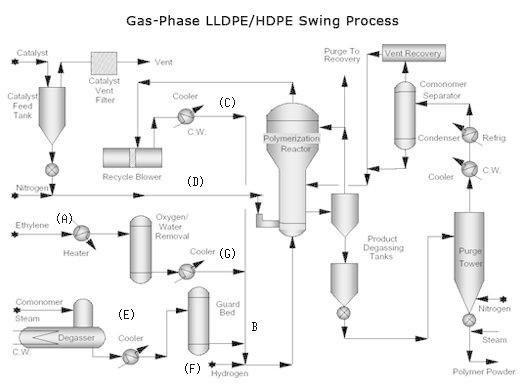
\includegraphics[width=0.8\textwidth,clip]{./Pics/hdpe_production_img2.jpg} 
     \caption{Gas Phase LLDPE/HDPE Swing Process Dow Chemical) fluxogram}\label{HDPE_Plant}
  \end{center}
\end{figure}

{\bf Gaseous Ethylene Stream:} prior to the removal of water and oxygen at the pressure vessel, gaseous ethylene $\left(\text{75}^{\circ}\text{C}\right)$ is heated up to 140$^{\circ}$C in a finned tube cross-flow heat exchanger (Fig.~\ref{HE_FlowPastHeatedCyclinder}, bottom). Fluid flowing in the tubes is mineral oil $\left(\href{http://twt.mpei.ac.ru/TTHB/HEDH/HTF-66.PDF}{\text{Therminol}\textregistered\text{66}} \text{ at 300}^{\circ}\text{C, with C}_{p}=2.57\text{ kJ.(kg.K)}^{-1}\right.$, 

$\left.\rho= 808.5\text{ kg.m}^{-3}, \kappa=0.095\text{W.(m.K)}^{-1}\text{ and }\mu=0.41\text{ mPa.s}\right)$. After the contaminants (water and oxygen) removal, the gaseous stream is refrigerated from 120$^{\circ}$C to 90$^{\circ}$C in a similar finned tube cross-flow heat exchanger (G, same mineral oil was used, but with temperature of 50$^{\circ}$C).  In order to support the design of such heat exchangers, specific technical information must to be obtained:
     \begin{enumerate}[a)]
        \item heat transfer from the tubes (containing $\text{Therminol}\textregistered\text{66}$) to the ethylene stream (A);
        \item heat transfer from the ethylene stream to the tubes (containing $\text{Therminol}\textregistered\text{66}$) (G);
        \item turbulence-induced mixing due to the pipes arrangement (Fig,~\ref{HE_FlowPastHeatedCyclinder} b-c) in both heat exchangers.        
     \end{enumerate}
     
     {\bf For this practical, we will focus on flow dynamics in the heat exchanger A. A systematic 2-D CFD study is suggested to assess the relevant parameters for this investigation, \ie drag forces, velocity, temperature and pressure profiles.}

     \section{Heat Exchanger A: Preliminary Analysis}
     In the design and optimisation of finned tube cross-flow heat exchangers, it is critical to have reliable information about flow dynamics (\ie spatial-distribution of pressure, temperature and velocity fields), turbulence energies and the impact of internals on them. Therefore, we should systematically study these variables by:
     \begin{enumerate}
       \item Model design and {\it quality assurance};
       \item Determine key-parameters for the cross-flow heat exchangers (overall drag and heat transfer).
     \end{enumerate}

     \subsection{Model and Software Quality Assurance (QA): Verification and Validation (\vv)}
                {\it Model and software quality assurance} encompass a set of procedures adopted by the CFD industry to ensure that models and software are in compliance with fundamental requirements, such as accuracy, range of confidence etc\footnote{\href{https://doi.org/10.1146/annurev.fluid.29.1.123}{P.J. Roache (1997) 'Quantification of Uncertainty in Computational Fluid Dynamics', Annual Review of Fluid Mechanics 29:123-160.}}. Model and software QA are the main means to assess the accuracy of computational simulations and comprise of two sets of procedures:
                \begin{enumerate}
                \item {\bf Verification} is a ``process of determining that a model implementation accurately represents the developer's conceptual description of the
model and the solution to the model''\footnote{\href{https://doi.org/10.1016/S0376-0421(02)00005-2}{W.L. Oberkampf and T.G. Trucano (2002) 'Verification and Validation in Computational Fluid Dynamics', Progress in Aerospace Sciences 38:209-272.}};
                   \item {\bf Validation} is a ``process of determining the degree to which a model is an accurate representation of the real world from the perspective of the intended uses of the model''$^{2}$;
                \end{enumerate}
                \vv procedures are critical tools to build confidence of numerical simulations. Before simulating flow and heat dynamics in the {\it Heat Exchanger A}, a \vv procedure should be designed to assess the initial accuracy of the model.
                \medskip

                {\it Flow past a cylinder} is a classical CFD \vv exercise and it is often used (a) to asses numerical accuracy (verification) and functionalities of models as the flow is steady and symmetric at low \Rey numbers and; (b) to validate against experimental solutions\footnote{\eg \href{https://doi.org/10.1017/S0022112064000544}{A.S. Grove {\it et al.} (1964) 'An Experimental Investigation of the Steady Separated Flow Past a Circular Cylinder', Journal of Fluid Mechanics 19:60-80}; \href{https://doi.org/10.1017/S0022112070001428}{S.C.R. Dennis and G. Chang (1970) 'Numerical Solutions for Steady Flow Past a Circular Cylinder at Reynolds Numbers up to 100', Journal Fluid Mechanics 42:471-489}; \href{https://doi.org/10.1017/S0022112059000829}{D.J. Tritton (1959) 'Experiments on the Flow Past a Circular Cylinder at Low Reynolds Numbers'  Journal Fluid Mechanics 6:547-567}; \href{https://doi.org/10.1017/S0022112061000950}{A. Roshko (1961) 'Experiments on the Flow Past a Circular Cylinder at Very High Reynolds Number', Journal of Fluid Mechanics 10:345-356}.}. At low Reynolds number (\Rey), any perturbation in the velocity boundary conditions is readily dissipated by viscous forces. However, as the \Rey increases, such perturbations may lead to fluid instabilities at the wake of the cylinder (also known as {\it 'vortex shedding'}), which may strongly impact on the fluid velocity and pressure fields and, therefore on momentum and heat transfers.

                
%%%
%%%  SUBSECTION: FLOW PAST A CYLINDER
%%%
     \subsubsection{Flow Past a Cylinder}\label{FlowPastCylinder}
     As a first step for \vv of the numerical model, perform numerical {\it flow past a cylinder} experiments (Fig.~\ref{HE_FlowPastHeatedCyclinder}a) with ethylene as the incompressible working fluid. Dimensions of the computational domain are:
     \begin{center}
       \begin{tabular}{c c c c c}
            D = 2.5 cm & L = 31.5 cm & L$_{1}$ = 11.5 cm & L$_{2}$ = 12.5 cm & H = 25.0 cm.  
       \end{tabular}
     \end{center}
     Simulations should be conducted with \Rey of \red{10, 120, 1000} and \red{5000}. 
 
     \begin{center}
       {\bf Procedure for Building the Geometry}
     \end{center}
     \red{From Dominc ... also do you know any fluid mechanics textbook(s) that contain(s) this subject (recommended reading) ? I guess 'cause of the heterogeneity of the group we can not make reference to Vlad's lecture notes.}

     \begin{shaded}
        \begin{center} \blue{\bf Tasks: } \end{center}
        \begin{enumerate}[a)]
           \item {\bf Verification:} determine the minimum mesh resolutions necessary for the numerical simulations (\ie grid that leads to mesh-independent solutions). Bear in mind that \Rey number (\ie flow regime) does affect the mesh resolution necessary to achieve mesh-independent solutions (see \blue{Tips} at the end of the document).
           \item {\bf Validation:} Determine drag coefficients around the cylinder for the performed simulations. Do they agree with expected values according to the \Rey numbers?
           \item {\bf Validation:} How do simulated velocity, pressure, vorticity and streamline profiles compare with either experimental or other numerical solutions? Comment on expected velocity, pressure and vorticity profiles (based on the literature) at different flow regimes (\ie laminar (low- and mid-\Rey) and turbulent flows).  
        \end{enumerate}  
     \end{shaded}
                     
%%%
%%%  SUBSECTION: FLOW PAST A HEATED CYLINDER
%%%
     \subsubsection{Flow Past a Heated Cylinder}\label{FlowPastHeatedCylinder}
     In order to investigate the heat exchange between the ethylene stream $\left(\text{75}^{\circ}\text{C}\right)$ and the cylinder, let's assume that the cylinder has constant temperature of 300$^{\circ}$C. Use the computational domain from Section~\ref{FlowPastCylinder} with \Rey of \red{10, 120, 1000} and \red{5000}. Here, assume that the {\bf fluid's density depends only on the temperature}.
     
     \begin{shaded}
        \begin{center} \blue{\bf Tasks: } \end{center}
        \begin{enumerate}[a)]
           \item {\bf Verification:} determine the minimum mesh resolutions necessary for the numerical simulations (\ie grid that leads to mesh-independent solutions). Bear in mind that \Rey number (\ie flow regime) does affect the mesh resolution necessary to achieve mesh-independent solutions.
           \item {\bf Validation:} Determine drag coefficient, heat transfer coefficient and Nusselt number around the cylinder for the performed simulations. Compare the $C_{D}$ with the expected value. Also, compare the obtained Nusselt number with the \red{ XX correlation:}
             \begin{displaymath}
               Nu = \frc{h L}{\kappa} = \red{k_{1} + k_{2}\Rey^{a}Pr^{b}},
             \end{displaymath}
             where $h$ is the inter-phase heat transfer coefficient, $L$ is the characteristic length, $\kappa$ is the conductive heat transfer coefficient and $Pr$ is the dimensionless Prandtl number.
           \item {\bf Validation:} How do simulated velocity, pressure, temperature, vorticity and streamline profiles compare with either experimental or other numerical solutions? Comment on expected temperature, velocity, pressure and vorticity profiles (based on the literature) at different flow regimes.
           \item Which flow regime provides the best heat diffusion? Why?
        \end{enumerate}  
     \end{shaded}


     \subsection{2-D Investigation of Heat Past a Bank of Heated Cylinders}
     Now, we should extend the initial model configuration to a bank of cylinders (all at constant temperature of 300$^{\circ}$C) to investigate the impact of turbulence induced by bluff bodies. You should allocate 9 cylinders in the domain in \underline{\bf both} staggered (Fig.~\ref{HE_FlowPastHeatedCyclinder}b) and non-staggered (Fig.~\ref{HE_FlowPastHeatedCyclinder}c) configurations. Assume that the {\bf fluid's density depends only on the temperature}. Distances L3-L7 should be defined to aim maximum heat diffusion. Simulations should be conducted for \Rey of 10, 80 and 120 for both cylinder configurations.
     
     \begin{shaded}
        \begin{center} \blue{\bf Tasks: } \end{center}
        \begin{enumerate}[a)]
           \item Determine the minimum mesh resolutions necessary for the numerical simulations (\ie grid that leads to mesh-independent solutions).
           \item Determine drag coefficient, heat transfer coefficient and Nusselt number around the cylinders for the performed simulations. 
           \item Show simulated velocity, pressure, temperature, vorticity and streamline profiles.
           \item Which flow regime and cylinder configuration provides the best heat diffusion? Why?
           \item Does the outlet temperature reach the expected value of 140$^{\circ}$C? If not, what would you suggest to improve heat diffusion?
        \end{enumerate}  
     \end{shaded}
     
      
     \begin{figure}[h]
         \vbox{ \hbox{\hspace{1cm}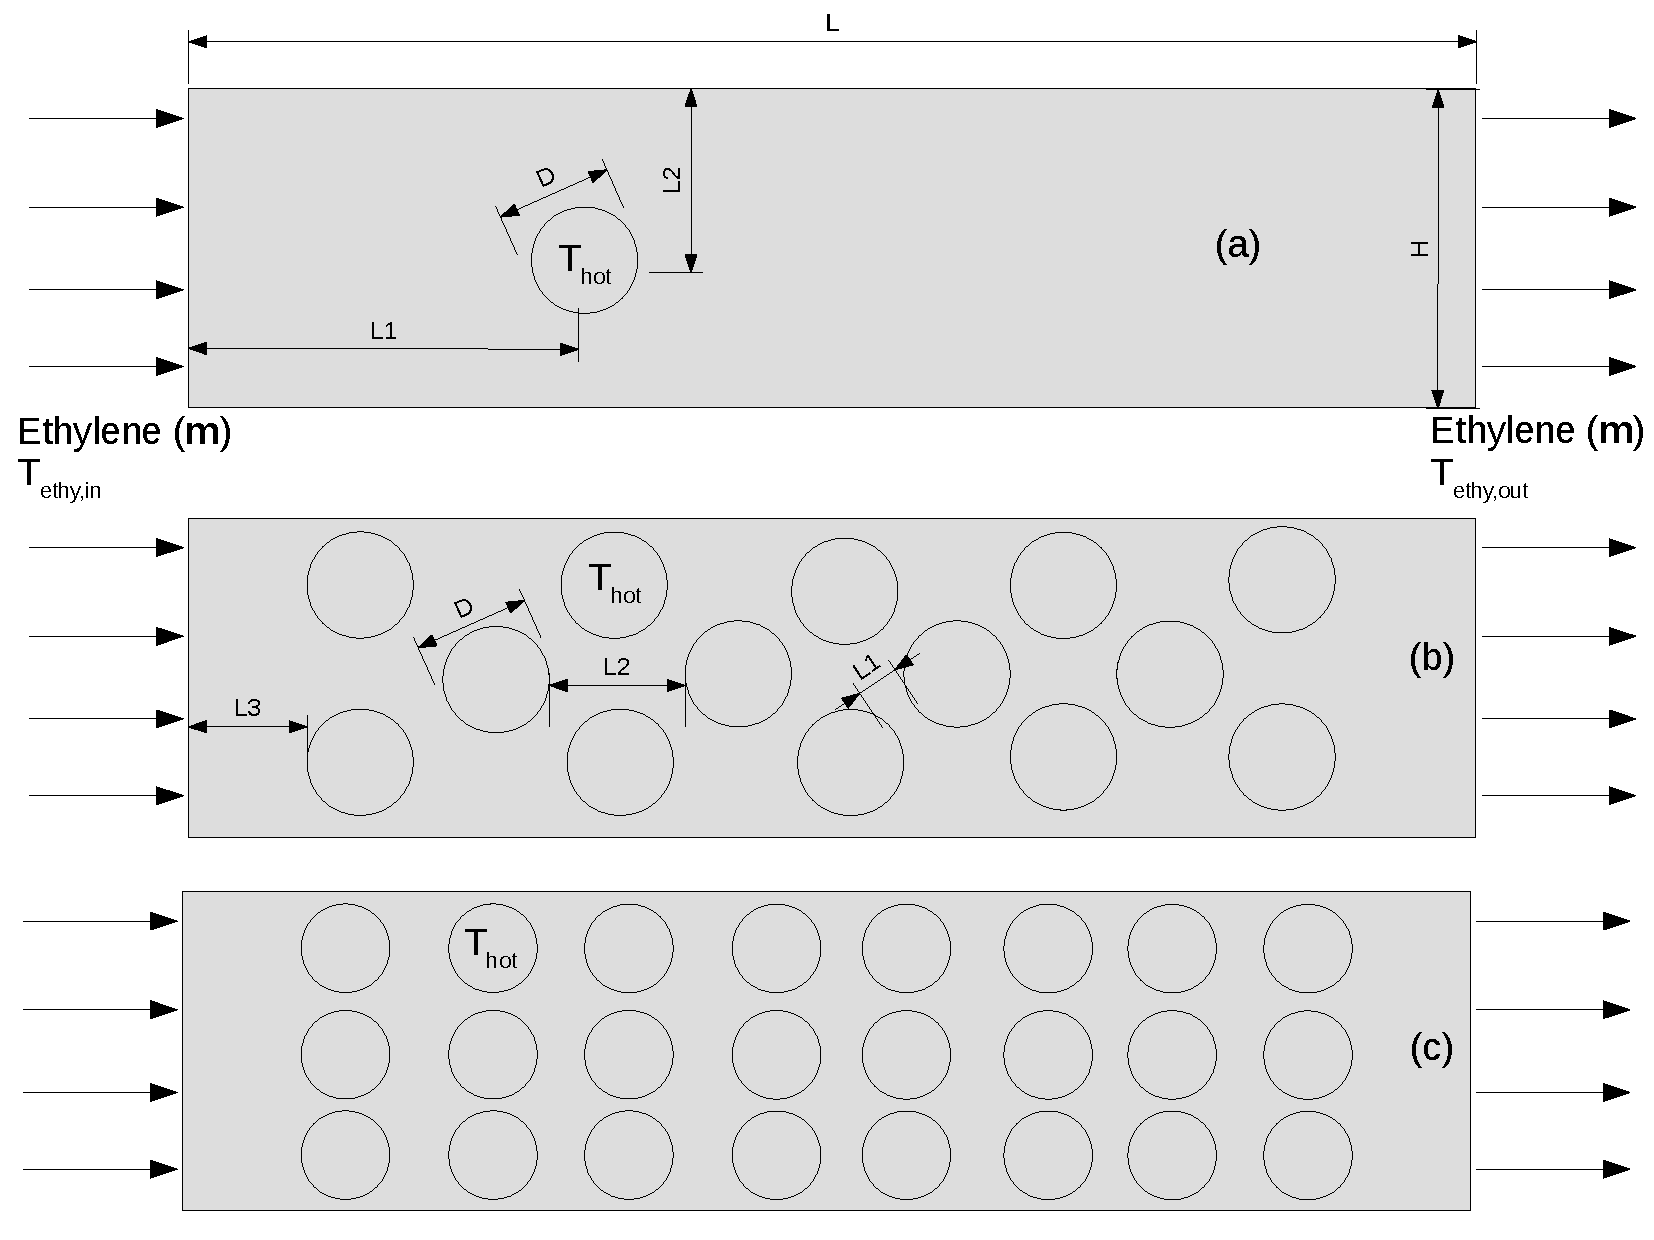
\includegraphics[width=0.7\textwidth,clip]{./Pics/HeatExchanger_2D.pdf}}
                \hbox{\hspace{3cm}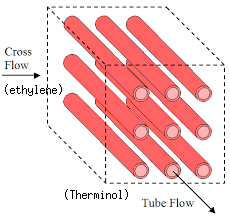
\includegraphics[width=0.5\textwidth,clip]{./Pics/HE_Finned.png}}}
         \caption{Flow past (heated) cylinder and banks of (heated) cylinders (top/middle). Cross-flow heat exchanger (bottom). }\label{HE_FlowPastHeatedCyclinder}
     \end{figure}

 \begin{comment}    
     
     \begin{enumerate}[1)]
        \item\label{1a} {\bf Flow past a heated cylinder:} A simplified 2D model involving ethylene gas flow past a heated cylinder (Fig.~\ref{HE_FlowPastHeatedCyclinder}, a) can be used to obtain information about drag forces and heat transfer (solid-fluid and fluid-fluid) that can later be used in the design and optimisation of the whole heat exchanger. 
        \item\label{1b} {\bf Flow past a bank of heated cylinders:} With the experience gained in (\ref{1a}), it is important to investigate the drag and heat transfer mechanisms in a bank of heated cylinders, i.e., the impact of such set of obstacles in the flow dynamics.
        \item\label{1c} Cross-flow heat exchanger (see \href{https://www.youtube.com/watch?v=-03gO3UwFeA}{https://www.youtube.com/watch?v=-03gO3UwFeA}): After the preliminary study (\ref{1a}-\ref{1b}) wrt optimal configuration of bank of heated cylinders, extend the model to 3D simulation and investigate flow dynamics and heat transfer rate.
     \end{enumerate}

     {\bf Tasks:}
     \begin{itemize}
        \item Initial geometry, mesh (unstructured) and set-up for 2D configurations described in \ref{1a}-\ref{1b};
        \item Gas compressibility assumptions: incompressible and compressible using PR-EOS;
        \item Investigation of drag around the cylinder(s) and the impact in the induced heat diffusion;
        \item Investigation of turbulence induced by the cylinder(s) through different models;
        \item Heat transfer efficiency in the \ref{1c}, temperature gradient in ethylene and oil (internal flow fluid) streams;
        \item Maybe optimal design for the heat exchanger.
     \end{itemize}

\end{comment}
\begin{comment}
Systems that will be investigated are:
\begin{enumerate}[A.]
  \item {\bf Gaseous Ethylene Stream:} prior to the removal of water and oxygen at the pressure vessel, gaseous ethylene $\left(\text{XX}^{\circ}\text{C, A}\right)$ is heated up in a finned tube cross flow heat exchanger (Fig.~\ref{HE_FlowPastHeatedCyclinder}, bottom). In order to support the design of such heat exchanger, specific technical information with respect to flow dynamics and heat transfer need to be obtained.
     \begin{enumerate}[i)]
        \item\label{1a} Flow past a heated cylinder: In order to obtain the appropriate parameters for the design of such heat exchanger, a simplified 2D model involving ethylene gas flow past a heated cylinder (Fig.~\ref{HE_FlowPastHeatedCyclinder}, top) can be used to obtain information about drag forces and heat transfer (solid-fluid and fluid-fluid) that can later be used in the design and optimisation of the whole heat exchanger. 
        \item\label{1b} Flow past a bank of heated cylinders: With the experience gained in (\ref{1a}), it is important to investigate the drag and heat transfer mechanisms in a bank of heated cylinders, i.e., the impact of such set of obstacles in the flow dynamics.
        \item\label{1c} Cross-flow heat exchanger (see \href{https://www.youtube.com/watch?v=-03gO3UwFeA}{https://www.youtube.com/watch?v=-03gO3UwFeA}): After the preliminary study (\ref{1a}-\ref{1b}) wrt optimal configuration of bank of heated cylinders, extend the model to 3D simulation and investigate flow dynamics and heat transfer rate.
     \end{enumerate}

     {\bf Tasks:}
     \begin{itemize}
        \item Initial geometry, mesh (unstructured) and set-up for 2D configurations described in \ref{1a}-\ref{1b};
        \item Gas compressibility assumptions: incompressible and compressible using PR-EOS;
        \item Investigation of drag around the cylinder(s) and the impact in the induced heat diffusion;
        \item Investigation of turbulence induced by the cylinder(s) through different models;
        \item Heat transfer efficiency in the \ref{1c}, temperature gradient in ethylene and oil (internal flow fluid) streams;
        \item Maybe optimal design for the heat exchanger.
     \end{itemize}

     \begin{figure}[h]
         \vbox{ \hbox{\hspace{1cm}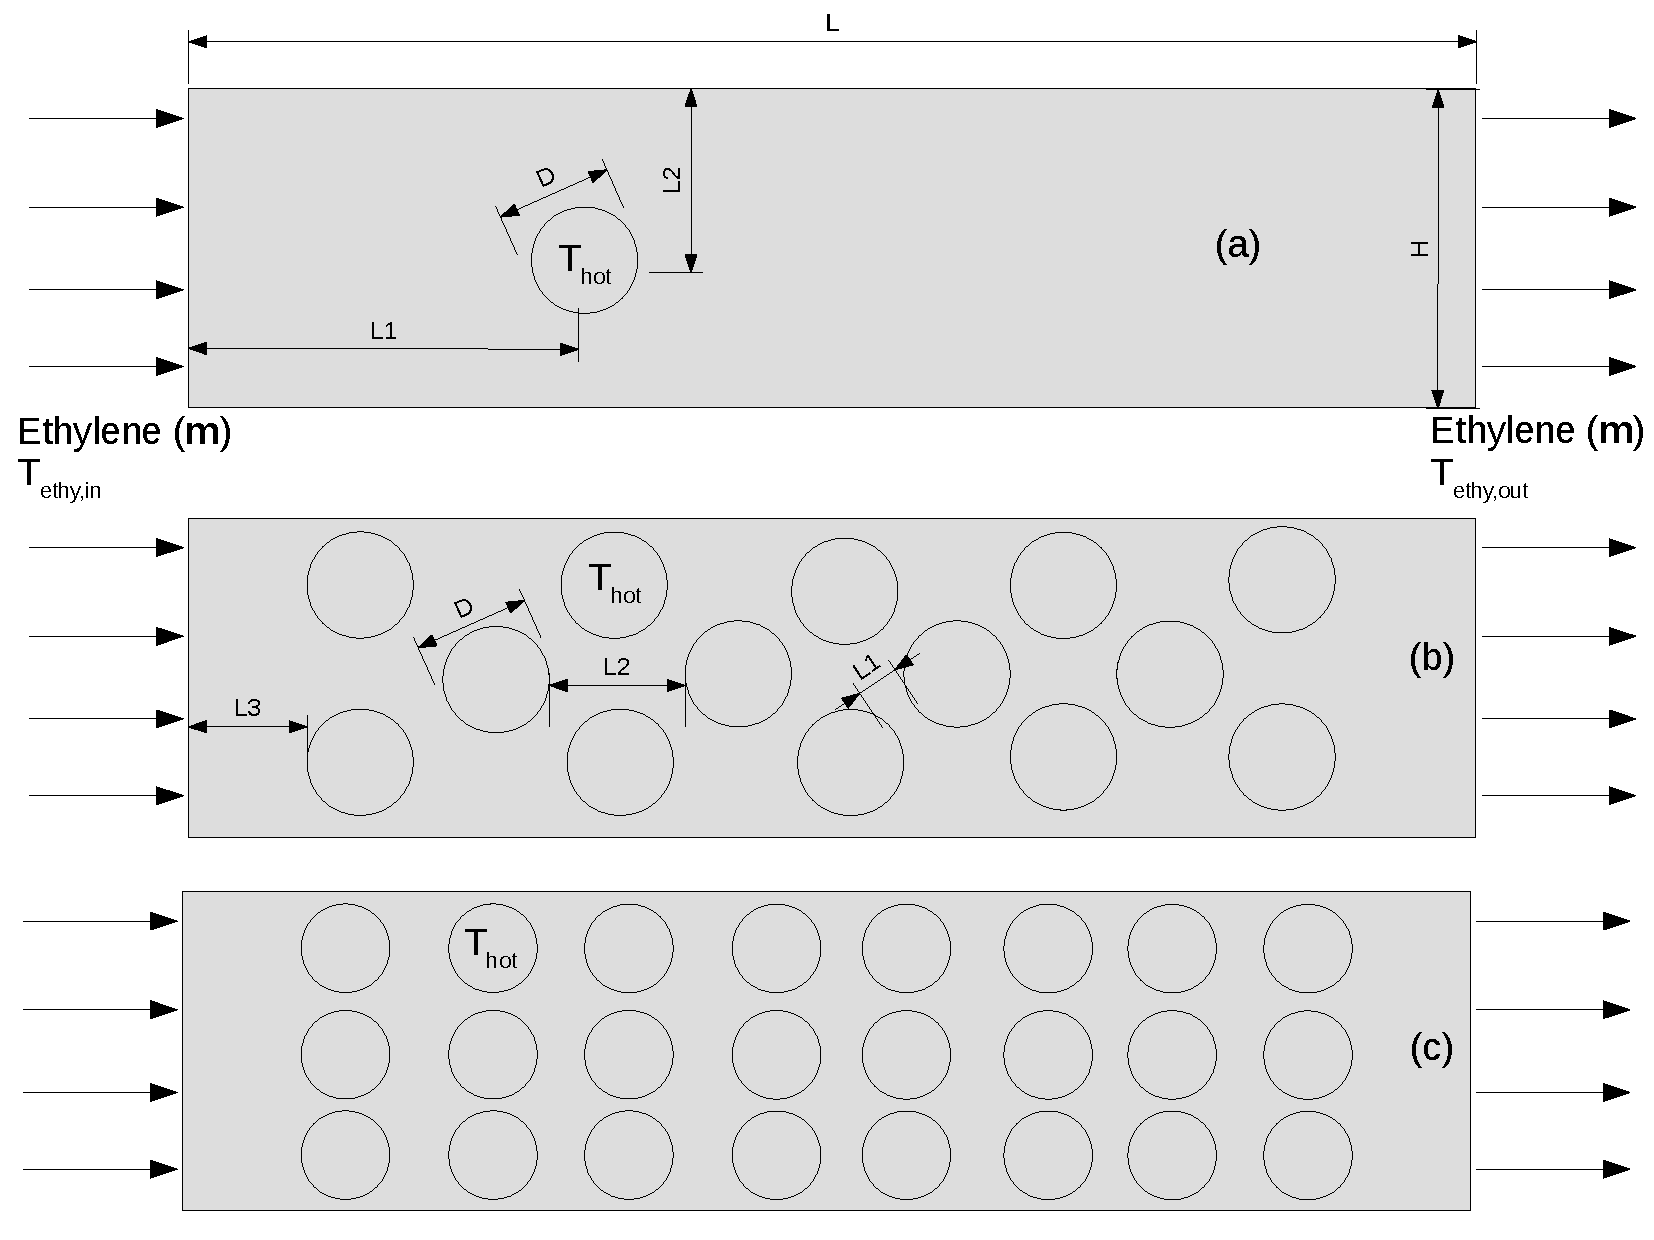
\includegraphics[width=0.7\textwidth,clip]{./Pics/HeatExchanger_2D.pdf}}
                \hbox{\hspace{3cm}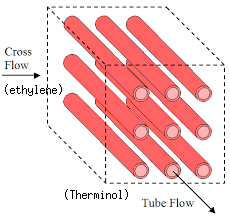
\includegraphics[width=0.5\textwidth,clip]{./Pics/HE_Finned.png}}}
         \caption{Flow past (heated) cylinder and banks of (heated) cylinders (top/middle). Cross-flow heat exchanger (bottom). }\label{HE_FlowPastHeatedCyclinder}
     \end{figure}
%%%
  \item {\bf Design of a Manifold Pipeline System:} four gaseous streams (B) are mixed before the polymerisation at the reactor in a hydraulic pipeline (Fig.~\ref{ManifoldPipeline}). The streams are:
     \begin{itemize}
        \item Ethylene (A) at XX$^{\circ}$C $\left(\dot{m}_{\text{ethyl}} = YY \text{kg.s}^{-1}\right)$;
        \item Hydrogen (F) at XY$^{\circ}$C $\left(\dot{m}_{\text{H}_{2}} = ZZ \text{kg.s}^{-1}\right)$;
        \item 2-Butene (comonomer, E) at XZ$^{\circ}$C $\left(\dot{m}_{\text{2-butene}} = ZY\right)$;
        \item Recycled (C, i.e., mixture of the above streams with composition of 15/60/25$\%$ in weight) at YZ$^{\circ}$C $\left(\dot{m}_{\text{rec}} = YX \text{kg.s}^{-1}\right)$.
     \end{itemize}
     
     {\bf Tasks:} The distance from the pre-processing units (A, C, E and F) to the reactor is of XX m and the reactor is placed in a platform at a height of YY m from the soil. You should design a manifold pipeline considering:
     \begin{itemize}
        \item Assume all pipelines are insulated and no heat is lost to the environment;
        \item Mesh analysis;
        \item The gaseous mixture should be injected into the polymerisation reactor at uniform temperature of $\left(kk\pm 5^{\circ}\text{C}\right)$. If the temperature resulting from the mixing does not reach the target, you may use an external heater (i.e., either prescribed heater temperature or flux);
        \item Turbulence models in the manifold pipeline system;
        \item Determine the optimal configuration for the manifold system that leads to the smallest pressure drop.
     \end{itemize}

     \begin{figure}[h]
         \vbox{ \hbox{\hspace{1cm}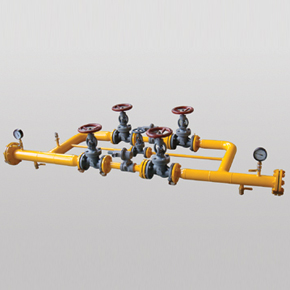
\includegraphics[width=0.7\textwidth,clip]{./Pics/ManifoldPipeline1.jpg}}
                \hbox{\hspace{3cm}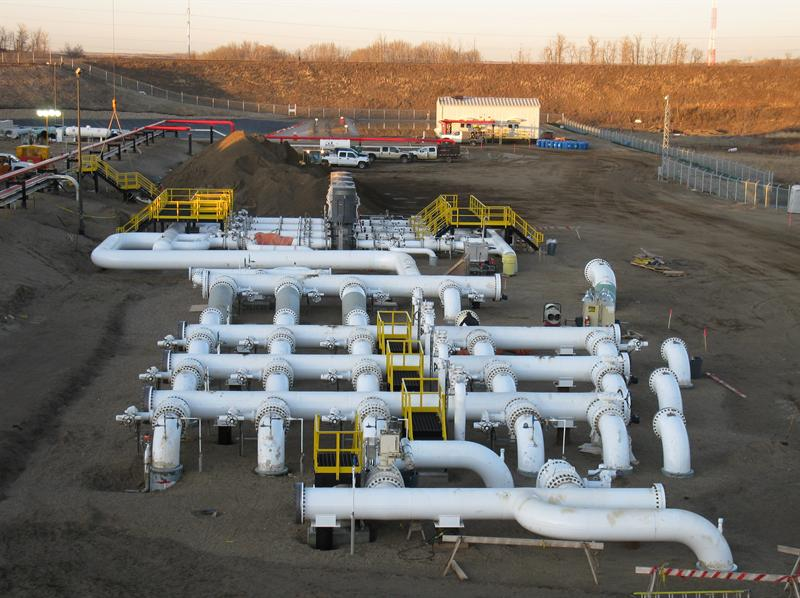
\includegraphics[width=0.5\textwidth,clip]{./Pics/ManifoldPipeline2.jpg}}}
         \caption{Manifold hydraulic pipeline (mixing of gases). }\label{ManifoldPipeline}
     \end{figure}
\end{enumerate}

\end{comment}






\clearpage
\begin{center} \Large{\bf Deliverables}\end{center}
\begin{enumerate}[1)]
  \item Write a report containing the {\bf summary of all performed numerical simulations} including,
       \begin{enumerate} [(a)]
          \item Initial geometry, mesh (unstructured), initial and boundary conditions;
          \item Mesh information and quality;
          \item Numerical schemes (\ie solution methods) and sub-models (\eg turbulence, heat transfer etc) used;
          \item Tasks requested.
     \end{enumerate} 
  
     \item Report should contain no more than (\underline{maximum}) 8 pages including bibliography and appendices (if any) -- see attached example, with the following structure (this {\bf does not} include plagiarism cover sheet):
       \begin{enumerate}
          \item Abstract: short summary of the main contents of the report including the main conclusions;
          \item Introduction: overview of the models (\ie conservative equations) used in the simulations and the relevance of the {\it flow past a cylinder} as a validation experiment for CFDs; 
          \item Simulation Setup: List of all relevant information wrt geometry, mesh, initial and boundary conditions and equations used;
          \item Results and Analysis;
          \item Concluding Remarks.
       \end{enumerate}


\item {\bf Prepare the report as \underline{PDF file} and submit it through {\it Turnitin} (with the appropriate plagiarism cover sheet) by Friday, November 24$^{\text{th}}$ 2017, noon at the latest. Also, submit a hard-copy of the report to the UG office by November 24$^{\text{th}}$, 15.00h.}
%
%\item Feedback will be provided on December YY$^{th}$ 2015.
%
\item Penalties for late or non-submission are as follows:
\begin{enumerate}%[(a)]
  \item Up to one week late, 2 CGS points deducted;
  \item Up to two weeks late, 3 CGS point deducted;
  \item More than two weeks late no marks awarded.
\end{enumerate}
If late or non-submission is due to medical or other circumstances out with your control you must submit a medical certificate or other formal evidence to the UG Office as soon as is practicable but no later than the end of Revision Week.

\item Note that the submitted work is part of the continuous assessment which will contribute 40$\%$ to your EG501V mark.

\end{enumerate}

       %%%
       %%% TIPS
       %%%
       
       \begin{shaded}
          \begin{center} \blue{\bf Tips} \end{center}
          \begin{enumerate}[i)]
             \item Although you do not need to show (in the report) plots and screen-shots on tests for verification (\eg mesh-independent solution, solution convergence, mass conservation, Y$^{+}$ for the turbulent flow simulations etc), you should perform all these tests as {\bf any failure may result in poor drag and heat transfer predictions};
             \item Ensure that residuals for the simulations are all set to 10$^{-5}$;
             \item For the solvers, use {\bf Standard} method for the {\bf pressure} field;
             \item \red{Dominic, any other tip?}
          \end{enumerate}
       \end{shaded}
       

\end{document}
